\documentclass[11pt,ngerman]{article}
\usepackage{geometry}
\usepackage[T1]{fontenc}
\usepackage[utf8]{inputenc}
\usepackage{babel}
\usepackage{lmodern}%get scalable font
\usepackage{titling}
\usepackage{relsize}
\usepackage{biblatex}
\usepackage{hyperref}
\usepackage{glossaries}
\usepackage{paralist}
\usepackage[table, dvipsnames]{xcolor}
\usepackage{booktabs}
\usepackage{tabularx}
\usepackage{float}
\restylefloat{table}
\usepackage{setspace}
\usepackage{multicol}
\usepackage{graphicx}

\usepackage{lipsum} % generates lorem ipsum => remove again when finished

\geometry{a4paper, top=25mm, left=25mm, right=25mm, bottom=20mm,
    headsep=10mm, footskip=12mm}

% Glossary
% Das Glossar definiert alle wichtigen Begriffe zur Sicherstellung einer einheitlichen Terminologie.
% Es sollen keine allgemeinen Begriffe erklärt werden, die den Adressaten bekannt sind (z. B. Java, CPU etc.).
% Glossareinträge müssen im Text verwendet werden damit diese im Glossar im Appendix \printglossary angezeigt werden
\makeglossaries
\loadglsentries{glossary} % loads glossary definitions from external file

\pretitle{\begin{center}\linespread{1.5}\huge}
    \posttitle{\par\end{center}\vspace{0.5em}}

\begin{document}

    \title{Tron Licht-Motorräder Computerspiel\\
        \vspace{1cm}
        Lösungsarchitektur \\
        \vspace{0.5cm}
        \small{}ZHAW  School of Engineering
        \vspace{1.5cm}
    }
    \author{
        Akca, Deniz\\
        \small{akcaden1@students.zhaw.ch}
        \and
        Holenstein, Christian\\
        \small{holenchr@students.zhaw.ch}
        \and
        Huber, Patrick\\
        \small{huberpa4@students.zhaw.ch}
        \and
        Iten, Mike\\
        \small{itenmik1@students.zhaw.ch}
        \vspace{1.5cm}
    }
   \date{\today}

    \maketitle
    \newpage

    \tableofcontents
    \listoftables
    \listoffigures
    \newpage

    % First section
    \section{Anwendungsfälle}
        Anwendungsfälle Übersicht:
        \begin{multicols}{2}
            \begin{itemize}
               \item Ein-  \& Ausloggen
               \item Registrieren
               \item Passwort zurücksetzen
               \item Lobby erstellen
               \item Freunde einladen
               \item Lobby beitreten
               \item Spiel starten
               \item Statistiken betrachten
               \item Authentifizierung
           \end{itemize}
        \end{multicols}

    \subsection{Anwendungsfalldiagramm}
        \begin{figure}[H]
            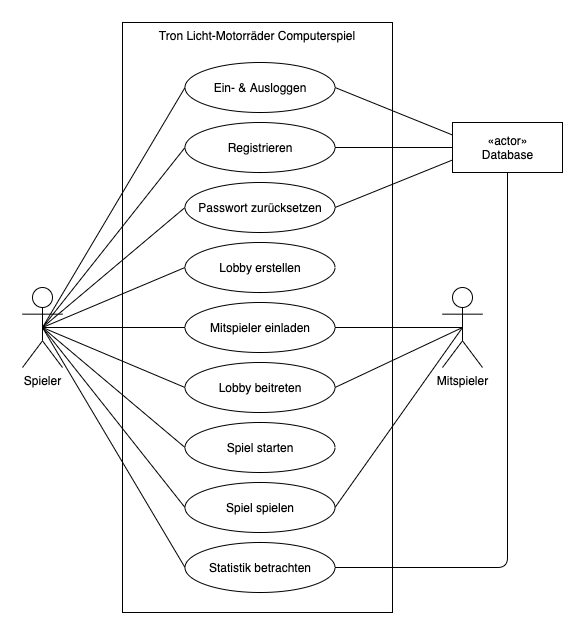
\includegraphics[scale=0.77]{figures/Use-case-modell.png}
            \caption{Anwendungsfalldiagramm - Tron Licht-Motorräder Computerspiel}
        \end{figure}

    \subsection{Use-Case-2}
    \lipsum[1]

    \section{Zusätzliche Anforderungen}

    \subsection{Funktionalität}
    \lipsum[1]

    \subsection{Benutzbarkeit}

    \subsection{Zuverlässigkeit}

    \subsection{Effizienz}

    \subsection{Änderbarkeit (Wartbarkeit)}

    \subsection{Internationalisierung}

    \subsection{Einschränkungen}

    \subsubsection{Designeinschränkungen}

    \subsubsection{Implementierungseinschränkungen}

    \subsubsection{Schnittstelleneinschränkungen}

    \section{Domänenmodell}

    \section{Softwarearchitektur}

    \section{Design-Artefakte}

    \section{Implementation}

    \section{Projektmanagement}


    % Appendix after this
     \newpage

    \section{Appendix}
    \textit{Hinweis: Glossar-Referenznummern sind Seitennummern}
    \printglossary

\end{document}

